\documentclass[]{article}
\usepackage{ctex}
\usepackage{amsmath}
\usepackage{amssymb}
\usepackage{setspace}
\usepackage{latexsym}
\usepackage{geometry}
\usepackage{graphicx}
\usepackage{listings}

\geometry{a4paper,left=2.5cm,right=2.5cm,top=2.5cm,bottom=2.5cm}
\begin{document}

\title{华强买瓜记}
\maketitle

\leftline{\Large{\textbf{摘要}}}
~\\
\indent 有一个人前来买瓜. 哥们儿, 这瓜多少钱一斤呐? 两块钱一斤. 我草, 你这瓜皮子是金子做的还是瓜粒子是金子做的? 你瞧瞧现在哪儿有瓜呀, 这都是大棚的瓜, 你嫌贵我还嫌贵呢. 给我挑一个. 行.\\
\indent 有一个人前来买瓜. 哥们儿, 这瓜多少钱一斤呐? 两块钱一斤. 我草, 你这瓜皮子是金子做的还是瓜粒子是金子做的? 你瞧瞧现在哪儿有瓜呀, 这都是大棚的瓜, 你嫌贵我还嫌贵呢. 给我挑一个. 行.有一个人前来买瓜. 哥们儿, 这瓜多少钱一斤呐? 两块钱一斤. 我草, 你这瓜皮子是金子做的还是瓜粒子是金子做的? 你瞧瞧现在哪儿有瓜呀, 这都是大棚的瓜, 你嫌贵我还嫌贵呢. 给我挑一个. 行.\\
~\\
\textbf{关键词}: 买瓜

\newpage

\section{问题重述}

\subsection{问题背景}
\begin{figure}[h]
    \centering
    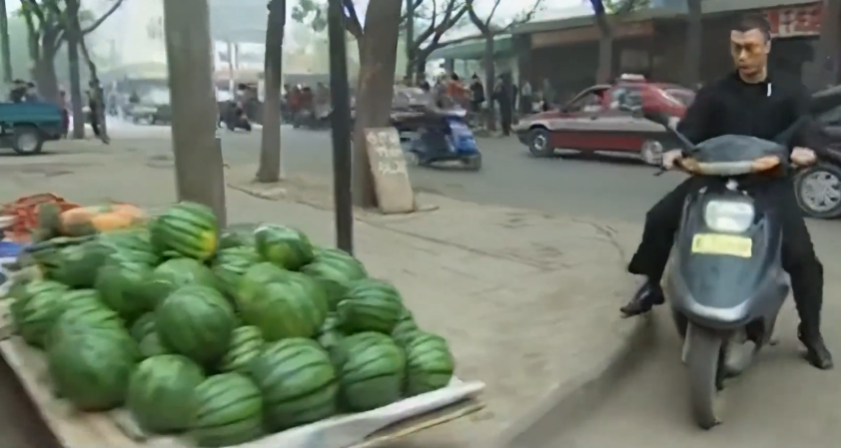
\includegraphics[width=3in]{buy.png}
    \caption{有一个人前来买瓜}
    \label{}
\end{figure}
\subsection{问题提出}

\indent 华强来干嘛?华强来干嘛?华强来干嘛?华强来干嘛?华强来干嘛?华强来干嘛?华强来干嘛?华强来干嘛?华强来干嘛?华强来干嘛?华强来干嘛?华强来干嘛?华强来干嘛?华强来干嘛?华强来干嘛?\\
\indent 华强来干嘛?华强来干嘛?华强来干嘛?华强来干嘛?华强来干嘛?华强来干嘛?华强来干嘛?华强来干嘛?华强来干嘛?华强来干嘛?华强来干嘛?华强来干嘛?华强来干嘛?华强来干嘛?华强来干嘛?华强来干嘛?华强来干嘛?\\

\section{问题分析}

\subsection{对情况一的分析}
\indent 华强来买瓜
\subsection{对情况二的分析}
\indent 华强来砍人
\subsection{对情况三的分析}
\indent 华强来找茬

\section{模型假设}

\begin{itemize}
    \item[(1)] 我是傻逼
    \item[(2)] 你也是傻逼
    \item[(3)] 我们都是傻逼
\end{itemize}

\section{符号说明}
~\\
\begin{table}[!h]
\centering
    \begin{tabular}{c|c}
    \hline
    \large{符号} & \large{含义} \\ 
    \hline
    $\mathcal{S}$ & 状态空间 \\
    $\mathcal{A}$ & 动作空间 \\
    $\mathcal{R}$ & 奖赏空间 \\
    $T(S' \mid S,A)$ & 状态转移函数 \\
    \hline
    \end{tabular}
\end{table}

\section{模型的建立、求解与检验}
\subsection{情形一}
\subsubsection{模型的准备}
\subsubsection{模型的建立}
\subsubsection{模型的求解}
\subsubsection{模型的检验}

\subsection{情形二}
\subsubsection{模型的准备}
\subsubsection{模型的建立}
\subsubsection{模型的求解}
\subsubsection{模型的检验}

\section{模型的评价}
\subsection{模型的优点}
\subsection{模型的缺点}

\begin{thebibliography}{99}
    \bibitem{ref1} www.bilibili.com
    \bibitem{ref2} www.zhihu.com 
    \bibitem{ref3} www.csdn.com
\end{thebibliography}

\newpage


\leftline{\Large{\textbf{附录}}}
\leftline{\textbf{附录一}: Hello world (Python)}
    \begin{lstlisting}
import nothing

def myprint():
    print("Hello world.")
    return
    
if __name__ == '__main__':
    myprint()
    \end{lstlisting}
    
~\\
\leftline{\textbf{附录二}: sort (Python)}
    \begin{lstlisting}
import nothing

def mysort(lst):
    return sorted(lst)
    
if __name__ == '__main__':
    a = [1,3,2]
    a = mysort(a)
    print(a)
    \end{lstlisting}

\end{document}
